\documentclass[titlepage]{article}

\usepackage[margin=1in]{geometry}
\usepackage{csquotes}
\usepackage{fancyhdr}
\usepackage{marginnote}
\usepackage{enumitem}
\usepackage{siunitx}
\usepackage[style=chem-acs]{biblatex}
\usepackage{pdfpages}
\usepackage{amsmath,amssymb}
\usepackage{subcaption}
\usepackage{mhchem}
\usepackage{chemfig}
\usepackage[hidelinks]{hyperref}

\MakeOuterQuote{"}

\fancypagestyle{main}{
    \fancyhf{}
    \fancyhead[L]{\leftmark}
    \fancyhead[R]{CHEM 22000}
    \fancyfoot[R]{Labalme\ \thepage}
}
\fancypagestyle{plain}{
    \fancyhf{}
    \renewcommand{\headrulewidth}{0pt}
}

\reversemarginpar

\setlist[itemize,3]{label={\scriptsize$\blacksquare$}}

\DefineBibliographyStrings{english}{bibliography={References}}

\setchemfig{atom sep=2em,fixed length=true,bond offset=3pt,cram width=3pt}
\setcharge{extra sep=3pt}

\newcommand{\R}{\mathbb{R}}
\newcommand{\e}[1][]{\text{e}^{#1}}

\usepackage{subfiles}

\addbibresource{../../main.bib}

\title{Spectral Data for Benzophenone}
\author{
    Steven Labalme\\
    \normalsize Lab Section 1A05
}

\begin{document}




\maketitle



\pagestyle{main}
\renewcommand{\leftmark}{Lab Assignment 1c}
\section*{Classification}
\begin{itemize}
    \item IUPAC name: Diphenylmethanone.
    \item Picture:
    \begin{center}
        \chemfig{*6(-=-(-(=[2]O)-[:-30]*6(=-=-=-))=-=)}
    \end{center}
\end{itemize}



\setitemize{label={--}}
\section*{Spectral Data}
\begin{enumerate}
    \item ${\color{white}hi}$
    \begin{figure}[H]
        \centering
        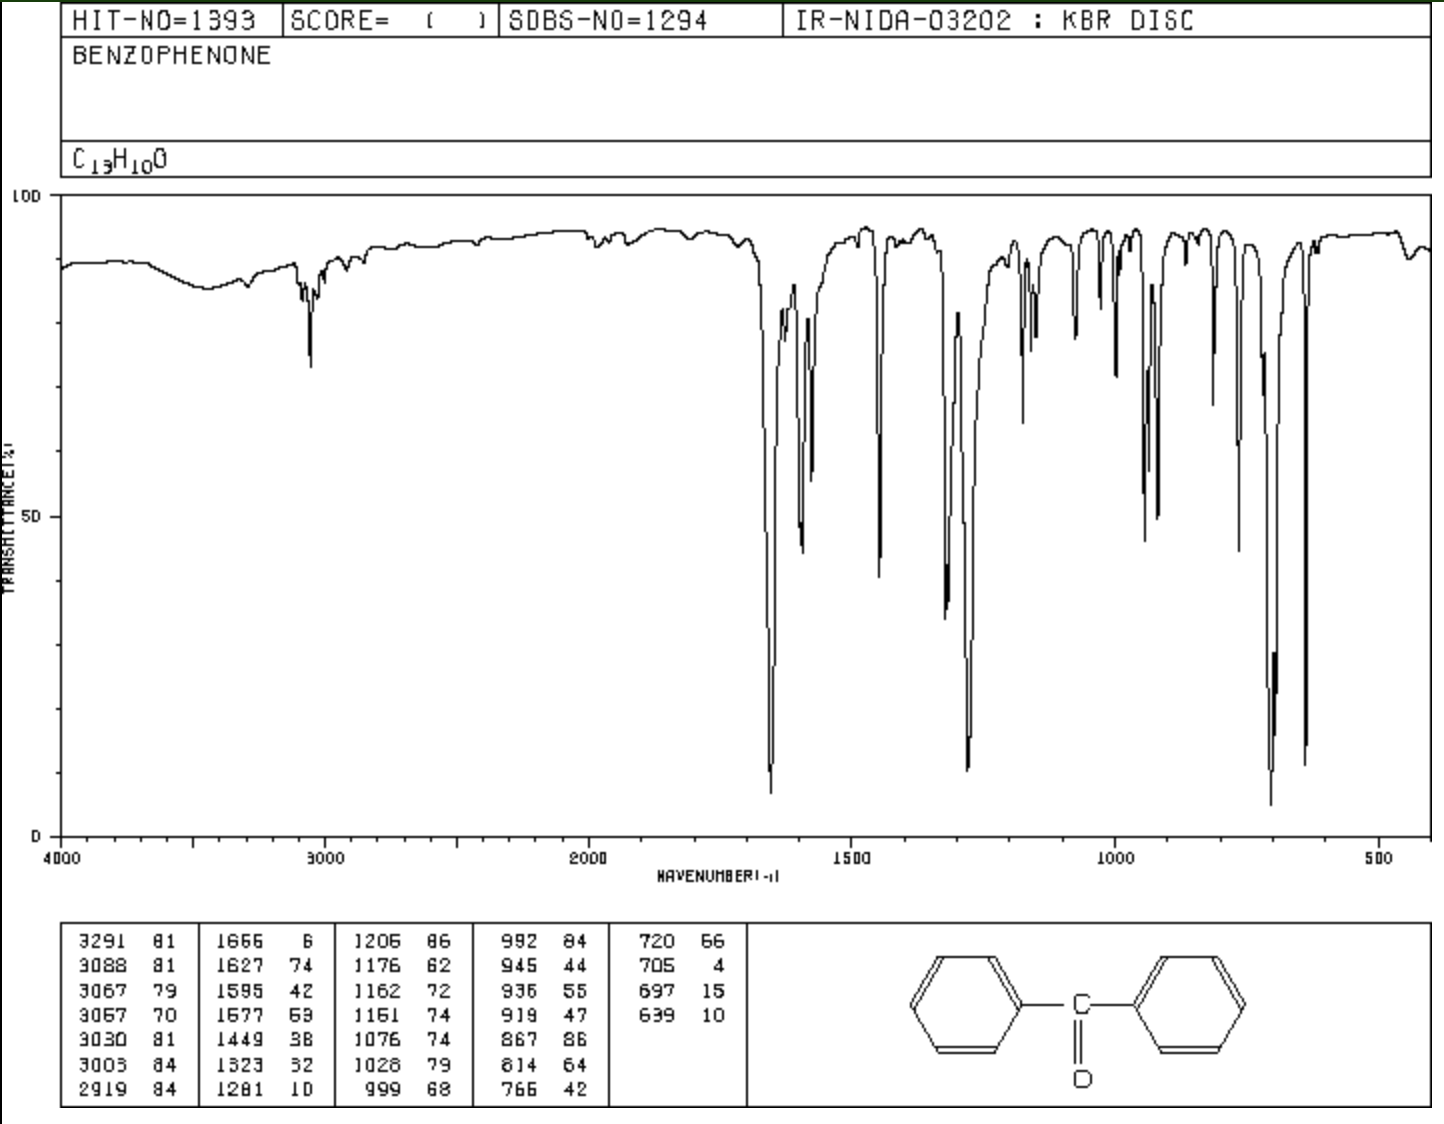
\includegraphics[width=0.8\linewidth]{../../ExtFiles/Benzophenone-IRSpectrum.png}
        \caption{IR spectrum of benzophenone\supercite{bib:Benzophenone-IRSpectrum}.}
        \label{fig:IRSpectrum}
    \end{figure}
    \pagebreak
    \item ${\color{white}hi}$
    \begin{figure}[H]
        \centering
        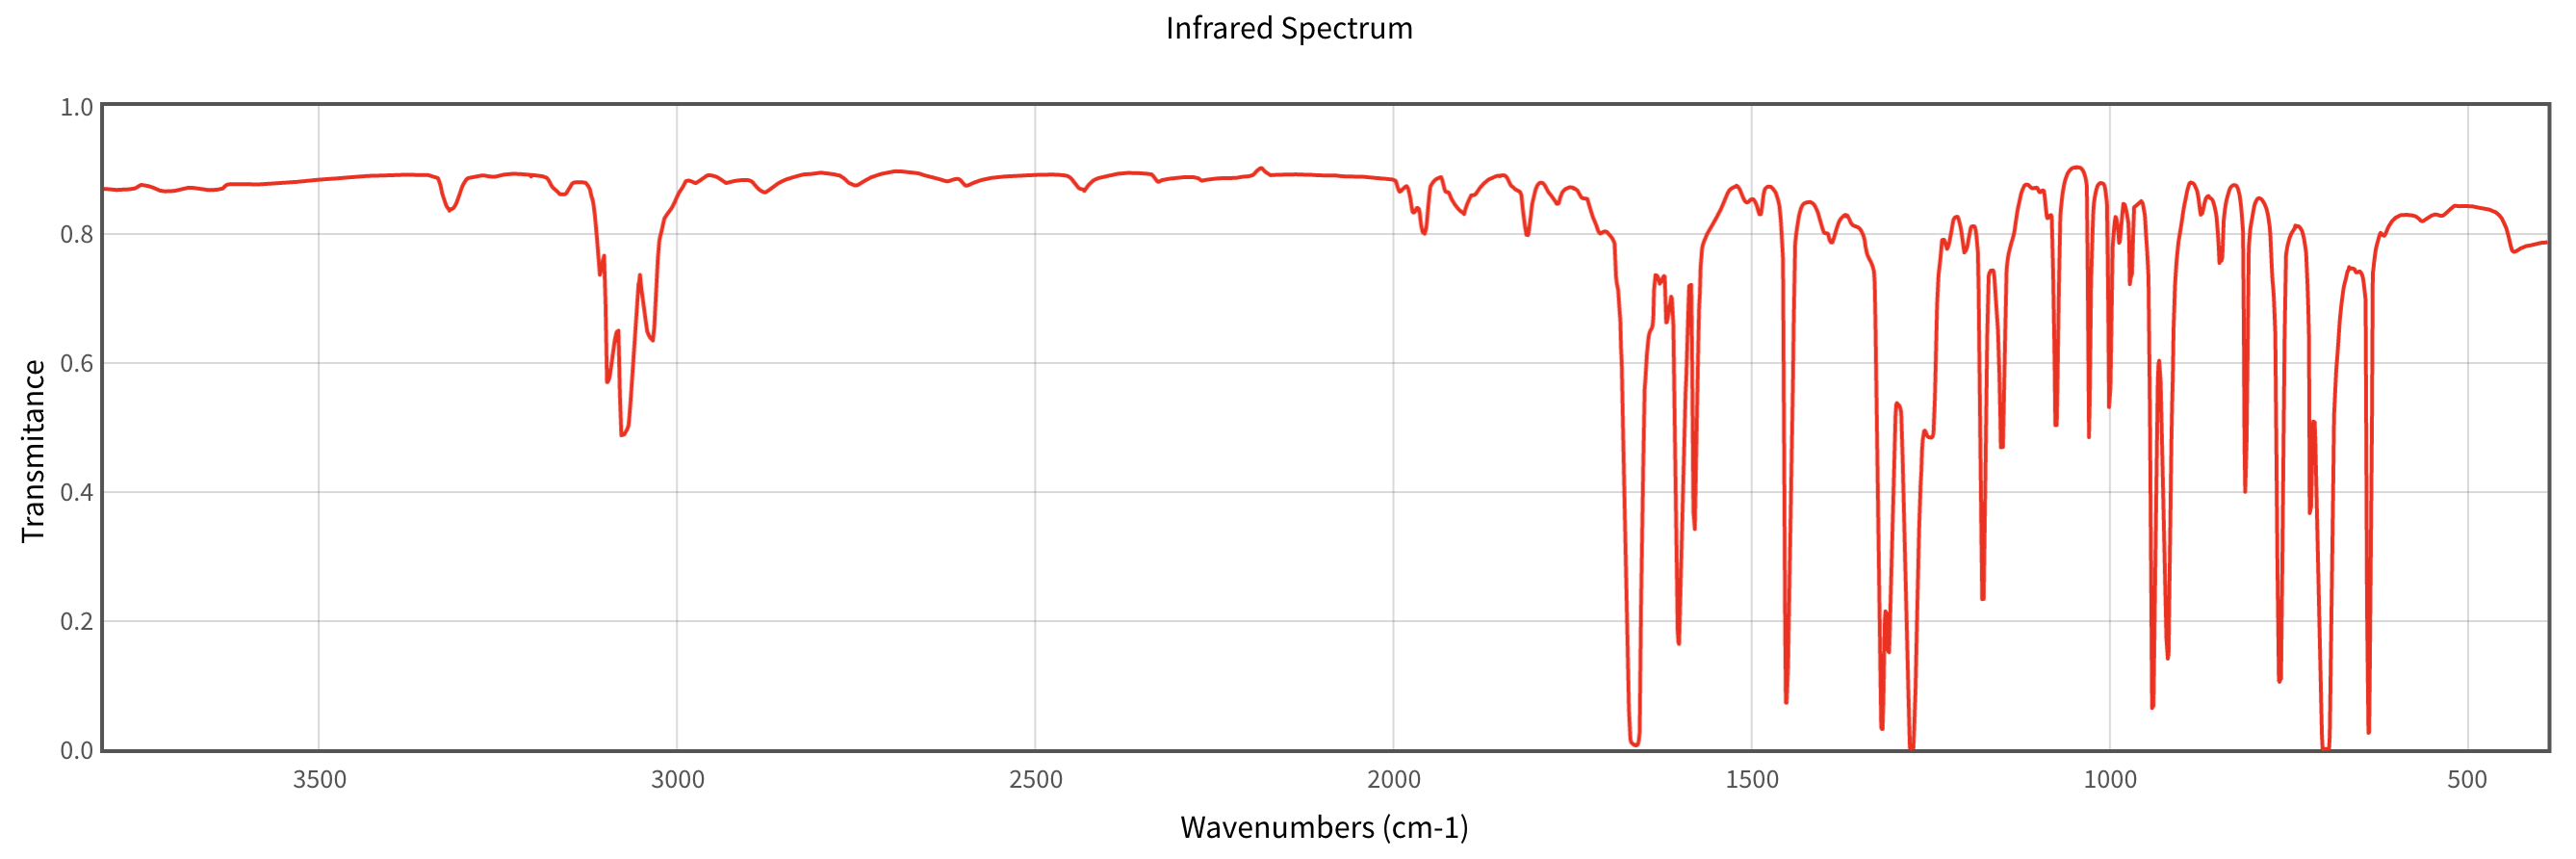
\includegraphics[width=0.8\linewidth]{../../ExtFiles/Benzophenone-IRSpectrum2.png}
        \caption{IR spectrum of benzophenone\supercite{bib:Benzophenone-IRSpectrum2}.}
        \label{fig:IRSpectrum2}
    \end{figure}
    \item Information in common:
    \begin{itemize}
        \item Molecule identifying information.
        \item The IR Spectrum from the SDBS database has data for much higher wavenumbers than the IR Spectrum from NIST.
    \end{itemize}
    \item Carbonyl data:
    \begin{itemize}
        \item Based on the IR spectra, benzophenone may have a carbonyl since we have a peak in the vicinity of $\SIrange{1710}{1735}{\per\centi\meter}$ although not strictly at it. This carbonyl is part of a ketone, and the wavenumber of the peak (from Figure \ref{fig:IRSpectrum}) is $\SI{1666}{\per\centi\meter}$. This is consistent with the fact that benzophenone does have a carbonyl.
    \end{itemize}
    \item Alcohol/amine data:
    \begin{itemize}
        \item Based on the IR spectra, benzophenone has neither an alcohol nor an amine since neither spectrum shows a peak at either $\SI{3400}{\per\centi\meter}$ or $\SI{3300}{\per\centi\meter}$, respectively. This is consistent with the fact that benzophenone has neither an alcohol nor an amine.
    \end{itemize}
    \item Alkyne/nitrile data:
    \begin{itemize}
        \item Based on the IR spectra, benzophenone has neither an alkyne nor a nitrile since neither spectrum shows a peak from $\SIrange{2100}{2300}{\per\centi\meter}$. This is consistent with the fact that benzophenone has neither an alkyne nor a nitrile.
    \end{itemize}
    \item Most prominent \ce{C-H} absorption peak:
    \begin{itemize}
        \item The $sp^2$ \ce{C-H} peak, just to the left of $\SI{3000}{\per\centi\meter}$, is the most prominent (and only) \ce{C-H} peak. This is consistent with the fact that benzophenone has only $sp^2$ \ce{C-H} bonds (no $sp^3$ or $sp$ \ce{C-H}) and, in fact, only $sp^2$ hybridized carbons.
    \end{itemize}
    \item Other prominent stretches:
    \begin{itemize}
        \item There appears to be some aromatic activity in the vicinity of $\SI{1500}{\per\centi\meter}$, owing to benzophenone's two aromatic rings. Consistent with the structure, there is not other distinguishing activity.
    \end{itemize}
\end{enumerate}
\newpage



\printbibliography




\end{document}